\chapter{Sistemas no inerciales; dinámica en la Tierra}\label{ch:b1:non-inertial-frames}

De pie en un autobús que gira a la izquierda, uno se inclina a la
derecha, empujado por una fuerza que nadie ejerce. Un cubo de agua que
gira sobre una plataforma ahueca su superficie en forma de cuenco. Bajo la
cúpula de un museo, un péndulo oscila durante horas y la línea de su
oscilación se desplaza despacio, unos grados por hora, como si la girara
una mano invisible. Ninguno de esos casos es una fuerza nueva: son el
aspecto que toman las \omterm{thm:b1:newton-dynamics:laws}{leyes de Newton} cuando el sistema en el que se
describe el movimiento está a su vez acelerado o girando. Este capítulo
muestra cómo se transforman velocidades y aceleraciones de un sistema a
otro, cómo se reparan las leyes de la dinámica añadiendo \emph{\omterm{thm:b1:non-inertial-frames:dynamics}{fuerzas de
inercia}} y qué hacen esas fuerzas en el sistema giratorio más importante
de todos: la Tierra.

\begin{omfigure}
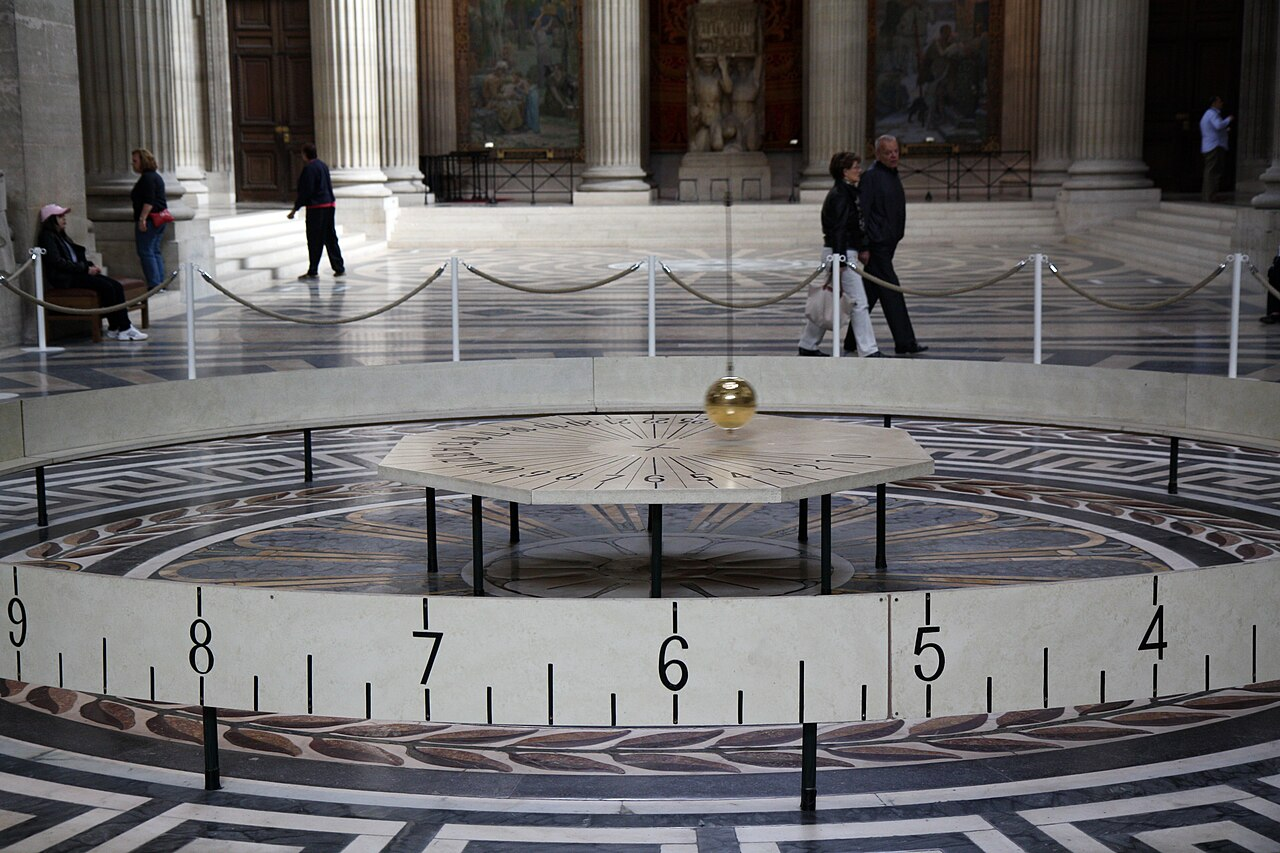
\includegraphics[width=0.55\linewidth]{images/book3/foucault-pendulum-pantheon.jpg}

{\small El \omterm{prop:b1:non-inertial-frames:foucault}{péndulo de Foucault} del Panteón de París, donde se colgó por primera vez en 1851: \qty{67}{m} de cable, una lenteja de \qty{28}{kg} y un plano de oscilación que gira respecto del suelo. Fotografía: Olga Khomitsevich, CC~BY~2.0.}
\end{omfigure}

\section{Cambiar de sistema: cinemática}

\begin{definition}[Movimiento relativo; sistema en traslación, en rotación]\label{def:b1:non-inertial-frames:frames}
\index{movimiento relativo}\index{sistema en traslación}\index{sistema en rotación}
Sean $\mathcal R$ un sistema (de origen $O$) y $\mathcal R'$ otro (de origen
$O'$) que se mueve respecto de él. $\mathcal R'$ está \emph{en traslación}
si sus ejes conservan direcciones fijas en $\mathcal R$ (todo punto de
$\mathcal R'$ tiene la velocidad de $O'$); está \emph{en rotación en torno
a un eje fijo} $\Delta$ si $\Delta$ es fijo en ambos sistemas y
$\mathcal R'$ gira en torno a él con la \omterm{cor:b1:point-kinematics:circular}{velocidad angular} $\Omega(t)$. La
velocidad y la aceleración de un punto $M$ \emph{relativas} a
$\mathcal R'$, $\vect v'$ y $\vect a'$, son las que mide un observador en
reposo en $\mathcal R'$.
\end{definition}

\begin{theorem}[Composición de velocidades y aceleraciones]\label{thm:b1:non-inertial-frames:composition}
\index{velocidad de arrastre}\index{aceleración de arrastre}\index{aceleración de Coriolis}
\begin{itemize}
  \item $\mathcal R'$ en traslación con velocidad $\vect v_{O'}$ y
        aceleración $\vect a_{O'}$:
        \[
        \vect v = \vect v' + \vect v_{O'}, \qquad \vect a = \vect a' + \vect a_{O'} .
        \]
  \item $\mathcal R'$ que gira en torno al eje fijo $\Delta$ con $\Omega$
        (vector $\vect\Omega = \Omega\vect e_z$ según el eje), siendo $H$ la
        proyección de $M$ sobre el eje:
        \[
        \vect v = \vect v' + \vect\Omega\wedge\vect{HM}, \qquad
        \vect a = \vect a' + \underbrace{\big(-\Omega^2\vect{HM} + \dot\Omega\,\vect e_z\wedge\vect{HM}\big)}_{\vect a_e}
        + \underbrace{2\vect\Omega\wedge\vect v'}_{\vect a_C} .
        \]
\end{itemize}
$\vect a_e$ es la \emph{\omterm{thm:b1:non-inertial-frames:composition}{aceleración de arrastre}} (la aceleración del punto
de $\mathcal R'$ que coincide con $M$: centrípeta hacia el eje si la
rotación es uniforme) y $\vect a_C = 2\vect\Omega\wedge\vect v'$ la
\emph{\omterm{thm:b1:non-inertial-frames:composition}{aceleración de Coriolis}}, presente solo cuando $M$ se mueve respecto
del sistema giratorio.
\end{theorem}

\begin{proof}
Traslación: $\vect{OM} = \vect{OO'} + \vect{O'M}$ con las componentes de
$\vect{O'M}$ en la base común; derívese dos veces. Rotación: úsense
\omterm{def:b1:point-kinematics:cylindrical}{coordenadas cilíndricas} en torno a $\Delta$ en $\mathcal R$, $(r, \theta, z)$,
y en $\mathcal R'$, $(r, \theta', z)$, con $\theta = \theta' + \int\Omega\,\dd t$.
Entonces \cref{thm:b1:point-kinematics:cylindrical} en $\mathcal R$ con
$\dot\theta = \dot\theta' + \Omega$:
$\vect v = \dot r\vect e_r + r(\dot\theta' + \Omega)\vect e_\theta + \dot z\vect e_z
= \vect v' + r\Omega\vect e_\theta$, y $r\Omega\vect e_\theta = \vect\Omega\wedge\vect{HM}$.
Para la aceleración, $\ddot\theta = \ddot\theta' + \dot\Omega$:
$\vect a = [\ddot r - r(\dot\theta' + \Omega)^2]\vect e_r + [r(\ddot\theta' + \dot\Omega)
+ 2\dot r(\dot\theta' + \Omega)]\vect e_\theta + \ddot z\vect e_z$; desarrollando
y agrupando, $\vect a = \vect a' - r\Omega^2\vect e_r + r\dot\Omega\vect e_\theta
+ 2\Omega(-r\dot\theta'\vect e_r + \dot r\vect e_\theta)$, y el último paréntesis
es $2\vect\Omega\wedge\vect v'$, pues $\vect e_z\wedge\vect e_r = \vect e_\theta$ y
$\vect e_z\wedge\vect e_\theta = -\vect e_r$.
\end{proof}

\begin{example}[Caminar sobre una plataforma giratoria]\label{ex:b1:non-inertial-frames:turntable}
En \cref{exo:b1:point-kinematics:12} se calculó la aceleración de una
persona que camina radialmente con rapidez $u$ sobre una plataforma que
gira con $\Omega$: $-ut\Omega^2\vect e_r
+ 2u\Omega\vect e_\theta$. En el lenguaje nuevo: aceleración relativa nula,
arrastre $-r\Omega^2\vect e_r$, Coriolis $2\vect\Omega\wedge u\vect e_r = 2u\Omega\vect e_\theta$.
\end{example}

\section{Dinámica en un sistema no inercial: las fuerzas de inercia}

\begin{theorem}[La ley de Newton en un sistema no inercial]\label{thm:b1:non-inertial-frames:dynamics}
\index{fuerza de inercia}\index{fuerza centrífuga}\index{fuerza de Coriolis}
En un sistema $\mathcal R'$ que no es inercial, el movimiento de un \omterm{def:b1:point-kinematics:frame}{punto
material} cumple
\[
m\vect a' = \sum\vect F + \vect F_e + \vect F_C, \qquad
\vect F_e = -m\vect a_e, \qquad \vect F_C = -m\vect a_C = -2m\vect\Omega\wedge\vect v' :
\]
la segunda ley de Newton vale siempre que a las fuerzas reales se añadan
la \emph{\omterm{prop:b1:newton-dynamics:drag}{fuerza de arrastre}} (para un \omterm{def:b1:non-inertial-frames:frames}{sistema en rotación} uniforme, la
\emph{\omterm{thm:b1:non-inertial-frames:dynamics}{fuerza centrífuga}} $+m\Omega^2\vect{HM}$, dirigida hacia fuera del
eje; para un \omterm{def:b1:non-inertial-frames:frames}{sistema en traslación}, $-m\vect a_{O'}$) y la \emph{\omterm{thm:b1:non-inertial-frames:dynamics}{fuerza de
Coriolis}}. Esas \emph{\omterm{thm:b1:non-inertial-frames:dynamics}{fuerzas de inercia}} no son interacciones: ningún
cuerpo las ejerce, no tienen reacción y desaparecen en un \omterm{thm:b1:newton-dynamics:laws}{sistema
inercial}.
\end{theorem}

\begin{proof}
$m\vect a = \sum\vect F$ en el \omterm{thm:b1:newton-dynamics:laws}{sistema inercial} $\mathcal R$; sustitúyase
$\vect a = \vect a' + \vect a_e + \vect a_C$ y pásense los dos términos al
segundo miembro.
\end{proof}

\begin{example}[El pasajero inclinado, la plomada]\label{ex:b1:non-inertial-frames:bus}
En un autobús que frena con $a = \qty{3.0}{m/s^2}$, una correa colgante
siente, en el sistema del autobús, la gravedad más una \omterm{thm:b1:non-inertial-frames:dynamics}{fuerza de inercia}
hacia delante $ma$: cuelga según la \emph{gravedad aparente}
$\vect g' = \vect g - \vect a_{O'}$, inclinada hacia delante un ángulo
$\arctan(a/g) = 17^\circ$. Un pasajero que quiera quedarse quieto ha de
inclinarse según esa vertical aparente. En un ascensor en caída libre,
$\vect g' = \vect 0$: ingravidez, vista desde dentro.
\end{example}

\begin{omfigure}
\begin{tikzpicture}[font=\small, x=1cm, y=1cm]
  % bus frame accelerating to the right (a): plumb bob tilts backward? braking: a points backward (left), bob tilts forward (right)
  \draw[thick] (-2.6,2.2) -- (2.6,2.2); \fill[pattern=north east lines] (-2.6,2.2) rectangle (2.6,2.4);
  \fill (0,2.2) circle (1.2pt);
  \draw[dashed] (0,2.2) -- (0,-0.2);
  \coordinate (B) at ($(0,2.2)+(-73:2.2)$);
  \draw[thick] (0,2.2) -- (B); \fill[omDef] (B) circle (3pt);
  \draw[-Stealth, omThm, very thick] (B) -- ++(0,-1.2) node[below] {$m\vect g$};
  \draw[-Stealth, omProp, very thick] (B) -- ++(0.9,0) node[right] {$-m\vect a_{O'}$};
  \draw[-Stealth, omExo, very thick] (B) -- ++(107:1.6) node[pos=0.6, left, xshift=-2pt] {$\vect T$};
  \draw (0,1.4) arc (-90:-73:0.8); \node at (0.3,1.15) {$\alpha$};
  \draw[-Stealth, thick] (-0.2,3.0) -- (-1.6,3.0); \node[below, font=\footnotesize] at (-0.9,2.95) {$\vect a_{O'}$ (frenado)};
  \draw[-Stealth, thick] (0.4,3.0) -- (1.8,3.0); \node[below, font=\footnotesize] at (1.1,2.95) {movimiento};
  \begin{scope}[xshift=7.4cm]
  \draw[-Stealth, thick] (0,-0.4) -- (0,3.2) node[above] {$\Delta$};
  \draw[omDef!40, dashed] (0,1.0) ellipse (2.2 and 0.5);
  \fill[omDef] (2.2,1.0) circle (2.5pt) node[below right] {$M$};
  \draw[-Stealth, omProp, very thick] (2.2,1.0) -- ++(1.3,0) node[right] {$m\Omega^2\vect{HM}$};
  \draw[-Stealth, omExo, very thick] (2.2,1.0) -- ++(0.3,-0.95) node[below] {$-2m\vect\Omega\wedge\vect v'$};
  \draw[-Stealth, omThm, thick] (2.2,1.0) -- ++(-0.6,0.75) node[above] {$\vect v'$};
  \draw[-Stealth, omDef] (0.6,2.9) arc (80:20:0.6) node[right] {$\Omega$};
  \end{scope}
\end{tikzpicture}

{\small \omterm{thm:b1:non-inertial-frames:dynamics}{Fuerzas de inercia}. Izquierda: en un autobús que frena, la
plomada cuelga según la gravedad aparente $\vect g - \vect a_{O'}$,
inclinada hacia delante. Derecha: en un sistema que gira con $\Omega$, un
\omterm{def:b1:point-kinematics:frame}{punto material} siente una \omterm{thm:b1:non-inertial-frames:dynamics}{fuerza centrífuga} que lo aleja del eje y, si se
mueve, una \omterm{thm:b1:non-inertial-frames:dynamics}{fuerza de Coriolis} perpendicular a su velocidad relativa.}
\end{omfigure}

\begin{example}[El cubo que gira]\label{ex:b1:non-inertial-frames:bucket}
El agua de un cubo que gira con $\Omega$ en torno a su eje vertical está en
reposo en el sistema giratorio bajo la gravedad y la \omterm{thm:b1:non-inertial-frames:dynamics}{fuerza centrífuga}: su
superficie libre es perpendicular a la gravedad aparente $\vect g' = -g\vect e_z +
\Omega^2r\vect e_r$ (la superficie de un fluido en reposo es normal al campo,
\cref{ch:b1:fluid-statics}). Su pendiente vale $\dd z/\dd r = \Omega^2r/g$,
de modo que $z = \Omega^2r^2/2g$: un paraboloide. A \qty{10}{rad/s}, el
borde de un cubo de \qty{10}{cm} queda \qty{5}{cm} por encima del centro
--- el principio del telescopio de espejo líquido, cuyo mercurio giratorio
toma exactamente la forma parabólica que necesita un espejo.
\end{example}

\begin{method}[Trabajar en un sistema no inercial]\label{met:b1:non-inertial-frames:method}
Elíjase el sistema en el que la pregunta resulte más sencilla (el
autobús, la plataforma, la Tierra); enumérense las fuerzas reales;
añádanse $-m\vect a_e$ y, si el cuerpo se mueve en el sistema,
$-2m\vect\Omega\wedge\vect v'$; después procédase como en
\cref{met:b1:newton-dynamics:method}. Cuidado: las \omterm{thm:b1:non-inertial-frames:dynamics}{fuerzas de inercia}
nunca aparecen en el balance energético como ``trabajo hecho por
alguien'' --- la \omterm{thm:b1:non-inertial-frames:dynamics}{fuerza de Coriolis}, perpendicular a $\vect v'$, no
trabaja; la \omterm{thm:b1:non-inertial-frames:dynamics}{fuerza centrífuga} deriva de la \omterm{def:b1:work-and-energy:conservative}{energía potencial}
$-\tfrac12 m\Omega^2r^2$ en un \omterm{def:b1:non-inertial-frames:frames}{sistema en rotación} uniforme.
\end{method}

\section{El sistema terrestre}

\begin{definition}[Sistemas geocéntrico y terrestre]\label{def:b1:non-inertial-frames:earth}
\index{sistema geocéntrico}\index{sistema terrestre}
El \emph{sistema geocéntrico} tiene su origen en el centro de la Tierra y
sus ejes apuntan a estrellas fijas; es inercial con excelente
aproximación para movimientos de un día o menos (su propia aceleración
alrededor del Sol vale solo \qty{6e-3}{m/s^2} y es casi uniforme sobre la
Tierra). El \emph{sistema terrestre}, ligado al suelo, gira respecto de él
en torno al eje polar con
\[
\Omega = \frac{2\pi}{\qty{86164}{s}} = \qty{7.29e-5}{rad/s} .
\]
\end{definition}

\begin{proposition}[El peso y la variación de $g$]\label{prop:b1:non-inertial-frames:weight}
\index{peso!y rotación terrestre}
En el \omterm{def:b1:non-inertial-frames:earth}{sistema terrestre}, un cuerpo en reposo siente la atracción
gravitatoria $m\vect{\mathcal G}$ y la \omterm{thm:b1:non-inertial-frames:dynamics}{fuerza centrífuga} $m\Omega^2\vect{HM}$; su
suma es lo que mide una balanza y lo que señala una plomada: el
\emph{peso} $m\vect g = m\vect{\mathcal G} + m\Omega^2\vect{HM}$. El término
centrífugo es máximo en el ecuador, $\Omega^2R = \qty{0.034}{m/s^2}$, un
$0.35\%$ de $g$; reduce $g$ de los polos al ecuador e inclina la vertical
respecto del centro de la Tierra hasta $0.1^\circ$ en las latitudes medias.
\end{proposition}

\begin{proof}
Aplíquese \cref{thm:b1:non-inertial-frames:dynamics} con $\vect v' = \vect 0$
(sin \omterm{thm:b1:non-inertial-frames:dynamics}{fuerza de Coriolis}); $\Omega^2R = (7.29\times10^{-5})^2 \times 6.37\times10^6$.
El ángulo de desviación se sigue del triángulo de $m\vect{\mathcal G}$ y la
\omterm{thm:b1:non-inertial-frames:dynamics}{fuerza centrífuga} (\cref{exo:b1:non-inertial-frames:6}).
\end{proof}

\begin{proposition}[La fuerza de Coriolis en la Tierra]\label{prop:b1:non-inertial-frames:coriolis}
En la latitud $\lambda$, un cuerpo que se mueve horizontalmente con
rapidez $v'$ siente una \omterm{thm:b1:non-inertial-frames:dynamics}{fuerza de Coriolis} horizontal de módulo
\[
F_C = 2m\Omega v'\sin\lambda ,
\]
dirigida hacia la \emph{derecha} del movimiento en el hemisferio norte y
hacia la izquierda en el sur, sea cual sea la dirección de marcha; un
cuerpo que cae verticalmente se desvía hacia el \emph{este} en $2m\Omega v'\cos\lambda$.
\end{proposition}

\begin{proof}
Descompóngase $\vect\Omega = \Omega(\cos\lambda\,\vect e_N + \sin\lambda\,\vect e_z)$
(norte y vertical local). Para $\vect v'$ horizontal, $-2m\vect\Omega\wedge\vect v'$
tiene una parte horizontal $-2m\Omega\sin\lambda\,\vect e_z\wedge\vect v'$ --- girada
$90^\circ$ en sentido horario respecto de $\vect v'$ visto desde arriba, si
$\lambda > 0$ --- y una parte vertical (despreciable frente a la
gravedad). Con $\vect v' =
-v'\vect e_z$ vertical: $-2m\Omega\cos\lambda\,\vect e_N\wedge(-v'\vect e_z) = 2m\Omega v'\cos\lambda\,
\vect e_E$, hacia el este.
\end{proof}

\begin{omfigure}
\begin{tikzpicture}[font=\small, x=1cm, y=1cm]
  \draw[omDef, thick] (0,0) circle (2.4);
  \draw[-Stealth, thick] (0,-3.0) -- (0,3.3) node[right] {$\vect\Omega$};
  \draw[dashed] (-2.6,0) -- (2.6,0);
  \coordinate (P) at (45:2.4);
  \fill[omThm] (P) circle (2pt);
  \draw[-Stealth, omThm, thick] (P) -- ++(45:1.0) node[right] {$\vect e_z$};
  \draw[-Stealth, omThm, thick] (P) -- ++(135:1.0) node[above left] {$\vect e_N$};
  \draw (0.9,0) arc (0:45:0.9); \node at (0.7,0.35) {$\lambda$};
  \draw[-Stealth, omExo, thick] (P) -- ++(45:0.45) ++(0,0) -- ++(0,0);
  \draw[-Stealth, omProp, very thick] (P) -- ++(0,1.2) node[above right] {$\vect\Omega$ (local)};
  \node[omProp, font=\footnotesize] at (3.0,1.2) {$\Omega\sin\lambda\,\vect e_z + \Omega\cos\lambda\,\vect e_N$};
  \begin{scope}[xshift=7.8cm]
  \draw[-Stealth] (-1.8,0) -- (2.0,0) node[right] {E};
  \draw[-Stealth] (0,-1.6) -- (0,2.0) node[above] {N};
  \draw[-Stealth, omThm, very thick] (0,0) -- (0,1.4) node[left] {$\vect v'$};
  \draw[-Stealth, omExo, very thick] (0,0.7) -- (1.1,0.7) node[right] {$\vect F_C$};
  \draw[omDef, thick, domain=0:1.5, samples=40] plot ({0.35*\x*\x},{\x});
  \node[font=\footnotesize] at (0.8,-0.9) {visto desde arriba, $\lambda > 0$};
  \end{scope}
\end{tikzpicture}

{\small Izquierda: en la latitud $\lambda$, el vector de rotación
terrestre tiene una componente vertical $\Omega\sin\lambda$ y otra hacia el
norte $\Omega\cos\lambda$. Derecha: visto desde arriba en el hemisferio
norte, un cuerpo que se mueve horizontalmente es empujado hacia su derecha
por la \omterm{thm:b1:non-inertial-frames:dynamics}{fuerza de Coriolis} y su \omterm{def:b1:point-kinematics:frame}{trayectoria} se curva en sentido horario.}
\end{omfigure}

\begin{example}[Fuerzas pequeñas, consecuencias grandes]\label{ex:b1:non-inertial-frames:coriolisnum}
Un tren a \qty{100}{km/h} en la latitud $45^\circ$: $a_C = 2 \times 7.29\times
10^{-5} \times 27.8 \times 0.71 = \qty{2.9e-3}{m/s^2}$, tres milésimas de
$g$ --- el carril derecho de una vía de sentido único se desgasta algo más
deprisa. El aire que fluye a \qty{20}{m/s} hacia un centro de bajas
presiones se desvía a la derecha durante todo el trayecto y acaba
girándolo en sentido antihorario: todos los ciclones del hemisferio norte
giran así, y todos los del sur al revés. Una piedra que cae por un pozo de
\qty{100}{m} en la latitud $45^\circ$ aterriza \qty{1.6}{cm} al este de la
plomada (\cref{exo:b1:non-inertial-frames:7}).
\end{example}

\begin{proposition}[El péndulo de Foucault]\label{prop:b1:non-inertial-frames:foucault}
\index{péndulo de Foucault}
Un péndulo que oscila con pequeña \omterm{def:b1:wave-propagation:signal}{amplitud} en la latitud $\lambda$
conserva su plano de oscilación frente a la sola rotación de la vertical
local del \omterm{def:b1:non-inertial-frames:earth}{sistema geocéntrico}: visto en el \omterm{def:b1:non-inertial-frames:earth}{sistema terrestre}, el plano
gira en \emph{sentido horario} (desde arriba, hemisferio norte) con la
\omterm{cor:b1:point-kinematics:circular}{velocidad angular} $\Omega\sin\lambda$, es decir una vuelta completa en
\[
T_F = \frac{\qty{23.93}{h}}{\sin\lambda} .
\]
\end{proposition}

\begin{proof}[Demostración parcial]
En el polo ($\lambda = 90^\circ$) el argumento es geométrico: sobre la
lenteja no actúa ninguna fuerza horizontal salvo la tensión, cuya
componente horizontal va según la oscilación, de modo que en el \omterm{def:b1:non-inertial-frames:earth}{sistema
geocéntrico} el plano de oscilación es fijo mientras la Tierra gira debajo
con $\Omega$; visto desde el suelo, gira con $-\Omega$. En la latitud
$\lambda$, la \omterm{thm:b1:non-inertial-frames:dynamics}{fuerza de Coriolis} horizontal vale
$-2m\Omega\sin\lambda\,\vect e_z\wedge\vect v'$: exactamente lo que produciría un
sistema que girase con $\Omega\sin\lambda$ en torno a la vertical local. En un
sistema que gire con el plano a $-\Omega\sin\lambda$, esa fuerza desaparece a
primer orden y el péndulo es un oscilador plano corriente; por tanto el
plano precesa con $\Omega\sin\lambda$ en el \omterm{def:b1:non-inertial-frames:earth}{sistema terrestre}. El cálculo
completo, con los términos de segundo orden despreciados, es el problema
de fin de semana.
\end{proof}

\begin{remark}[Las mareas, en dos líneas]\label{rem:b1:non-inertial-frames:tides}
\index{mareas}
En el sistema del centro de la Tierra, que cae libremente hacia la Luna,
la atracción lunar no es uniforme: algo mayor en la cara próxima y menor
en la lejana. La diferencia, del orden de $2GM_{\text{Luna}}R/d^3
\approx \qty{1e-6}{m/s^2}$, estira los océanos en dos abultamientos ---
dos mareas al día --- y la contribución del Sol, un $46\%$ de la lunar,
produce las mareas vivas y muertas según se alineen o se crucen las dos
(\cref{exo:b1:non-inertial-frames:12}).
\end{remark}

\section{Ejercicios}

\begin{exercise}[$\star$]\label{exo:b1:non-inertial-frames:1}
Una plomada cuelga en un coche que acelera a \qty{2.5}{m/s^2}: ángulo con
la vertical y tensión en unidades de $mg$. ¿Y el mismo coche frenando al
mismo ritmo?
\end{exercise}

\begin{exercise}[$\star$]\label{exo:b1:non-inertial-frames:2}
Un niño se sienta a \qty{3.0}{m} del eje de un tiovivo que da una vuelta
cada \qty{4.0}{s}. Aceleración centrífuga en el sistema giratorio, como
fracción de $g$; ¿qué fuerza real la proporciona?
\end{exercise}

\begin{exercise}[$\star$]\label{exo:b1:non-inertial-frames:3}
Calcúlense la \omterm{cor:b1:point-kinematics:circular}{velocidad angular} $\Omega$ de la Tierra, la aceleración
centrífuga en el ecuador y su fracción de $g$. ¿Con qué periodo de
rotación saldrían despedidos los objetos del ecuador?
\end{exercise}

\begin{exercise}[$\star$]\label{exo:b1:non-inertial-frames:4}
Un tren de \qty{400}{t} circula a \qty{100}{km/h} en la latitud $45^\circ$.
\omterm{thm:b1:non-inertial-frames:composition}{Aceleración de Coriolis} y fuerza lateral sobre los carriles; ¿qué carril
recibe el empuje si va hacia el norte? ¿Y hacia el este?
\end{exercise}

\begin{exercise}[$\star\star$]\label{exo:b1:non-inertial-frames:5}
Un cubo de \qty{10}{cm} de radio gira a \qty{2.0}{rad/s} y después a
\qty{10}{rad/s}. Elevación del agua en el borde respecto del centro. ¿Por
qué es un buen espejo de telescopio un baño de mercurio giratorio?
\end{exercise}

\begin{exercise}[$\star\star$]\label{exo:b1:non-inertial-frames:6}
Muéstrese que la plomada en la latitud $\lambda$ se desvía del centro de
la Tierra en aproximadamente $\Omega^2R\sin\lambda\cos\lambda/g$ radianes, y
calcúlese en $45^\circ$ en minutos de arco. ¿Cuánto menor es $g$ en el
ecuador que en el polo solo por la rotación?
\end{exercise}

\begin{exercise}[$\star\star$]\label{exo:b1:non-inertial-frames:7}
Una piedra cae desde el reposo por un pozo de \qty{100}{m} en la latitud
$45^\circ$. Trátese la \omterm{thm:b1:non-inertial-frames:composition}{aceleración de Coriolis} $2\Omega v\cos\lambda$ (hacia
el este) como una pequeña perturbación con $v = gt$; intégrese dos veces
para hallar la desviación hacia el este en el fondo. ¿Por qué hacia el este?
\end{exercise}

\begin{exercise}[$\star\star$]\label{exo:b1:non-inertial-frames:8}
Periodo de precesión de un \omterm{prop:b1:non-inertial-frames:foucault}{péndulo de Foucault} en París ($\lambda = 48.9^\circ$),
en el polo y en el ecuador. ¿Qué ángulo gira el plano en una hora en París?
\end{exercise}

\begin{exercise}[$\star\star$]\label{exo:b1:non-inertial-frames:9}
El aire fluye a \qty{20}{m/s} hacia un centro de bajas presiones a
$45^\circ$ norte. \omterm{thm:b1:non-inertial-frames:composition}{Aceleración de Coriolis}; ¿en qué sentido acaba girando
el aire alrededor del centro? ¿Por qué no obedecen esta regla los
remolinos pequeños (un desagüe, un tornado)?
\end{exercise}

\begin{exercise}[$\star\star\star$]\label{exo:b1:non-inertial-frames:10}
Un globo de helio atado a un hilo flota dentro de un coche. Cuando el
coche acelera hacia delante, ¿hacia dónde se inclina el globo?
Explíquese con la gravedad aparente y el empuje.
\end{exercise}

\begin{exercise}[$\star\star\star$]\label{exo:b1:non-inertial-frames:11}
Una estación espacial es un anillo de \qty{100}{m} de radio que gira para
dar $1g$ de gravedad artificial en el borde. ¿Periodo de rotación? Un
astronauta camina por el borde a \qty{1.5}{m/s}: \omterm{thm:b1:non-inertial-frames:composition}{aceleración de Coriolis} y
su efecto sobre el peso aparente al caminar a favor y en contra de la
rotación. Deja caer una pelota desde \qty{2.0}{m}: ¿a qué distancia de sus
pies cae, aproximadamente?
\end{exercise}

\begin{exercise}[$\star\star\star$]\label{exo:b1:non-inertial-frames:12}
Muéstrese que la diferencia entre la aceleración gravitatoria de la Luna
en el centro de la Tierra y en el punto de la superficie más cercano a la
Luna vale aproximadamente $2GM_Mr/d^3$ ($r$ el radio terrestre, $d$ la
distancia Tierra--Luna); calcúlese, y lo mismo para el Sol; dedúzcase el
cociente entre las mareas solares y las lunares.
\end{exercise}

\section{Problema: el péndulo de Foucault}

\begin{problem}[{Problema de fin de semana --- una lenteja de 28
kilogramos en un cable de 67 metros bajo una cúpula: por qué gira su plano
de oscilación, a qué ritmo, qué demuestra y qué fuerza tan pequeña lo hace}]
\label{pb:b1:non-inertial-frames:1}
En 1851, un péndulo de longitud $\ell = \qty{67}{m}$ y masa $m = \qty{28}{kg}$
osciló bajo la cúpula del Panteón de París, en la latitud $\lambda =
48.85^\circ$, con una \omterm{def:b1:wave-propagation:signal}{amplitud} de unos $x_0 = \qty{3.0}{m}$. $\Omega =
\qty{7.29e-5}{rad/s}$, $g = \qty{9.81}{m/s^2}$.

\medskip
\noindent\textbf{Parte I --- El péndulo como tal.}
\begin{enumerate}
  \item Periodo de las \omterm{prop:b1:work-and-energy:stability}{pequeñas oscilaciones}; compruébese que la \omterm{def:b1:wave-propagation:signal}{amplitud}
        es pequeña ($x_0/\ell$).
  \item Rapidez máxima de la lenteja y su altura máxima sobre el punto más
        bajo.
  \item Tensión en el punto más bajo, en unidades de $mg$.
  \item Estímese el arrastre del aire sobre la lenteja a la rapidez máxima
        (ley cuadrática, $C_xS \approx \qty{0.05}{m^2}$, $\rho = \qty{1.2}{kg/m^3}$)
        y compárese con la fuerza recuperadora máxima $m\omega_0^2x_0$.
  \item ¿Por qué un cable largo y una lenteja pesada? (Dos razones, una
        sobre el periodo y otra sobre el amortiguamiento.)
\end{enumerate}

\medskip
\noindent\textbf{Parte II --- En el polo.}
Imagínese el mismo péndulo en el polo norte.
\begin{enumerate}[resume]
  \item En el \omterm{def:b1:non-inertial-frames:earth}{sistema geocéntrico}, enumérense las fuerzas sobre la lenteja
        y muéstrese que nada puede girar su plano de oscilación.
  \item Dedúzcase qué le ve hacer al plano un observador de pie sobre el
        hielo, y en cuánto tiempo vuelve a su dirección inicial.
  \item Descríbase la \omterm{def:b1:point-kinematics:frame}{trayectoria} de la lenteja sobre el suelo (una
        roseta): ¿cuántos pétalos en un día?
\end{enumerate}

\medskip
\noindent\textbf{Parte III --- En la latitud $\lambda$: el término de Coriolis.}
Úsense ejes locales: $x$ al este, $y$ al norte, $z$ hacia arriba;
oscilaciones pequeñas, de modo que el movimiento es casi horizontal,
$\vect v' \approx (\dot x, \dot y, 0)$; la fuerza recuperadora vale
$-m\omega_0^2(x, y, 0)$ con $\omega_0 = \sqrt{g/\ell}$.
\begin{enumerate}[resume]
  \item Escríbase $\vect\Omega$ en estos ejes.
  \item Calcúlese $-2m\vect\Omega\wedge\vect v'$ y consérvense sus
        componentes horizontales; muéstrese que solo interviene
        $\Omega\sin\lambda$.
  \item Escríbanse las dos ecuaciones del movimiento para $x$ e $y$;
        hágase $\omega_F = \Omega\sin\lambda$ y compárese $\omega_F$ con $\omega_0$.
  \item Introdúzcase $u = x + jy$ y muéstrese que $\ddot u + 2j\omega_F\dot u +
        \omega_0^2u = 0$.
  \item Pruébese con $u = \eu^{j\alpha t}$: hállense los dos valores de
        $\alpha$ y muéstrese que, si $\omega_F \ll \omega_0$, valen $\alpha \approx \pm\omega_0
        - \omega_F$.
  \item Dedúzcase que $u \approx \eu^{-j\omega_Ft}(A\eu^{j\omega_0t} + B\eu^{-j\omega_0t})$
        e interprétese el factor $\eu^{-j\omega_Ft}$: ¿en qué sentido y a qué
        ritmo gira el plano de oscilación?
  \item Calcúlense el periodo de precesión en París y el ángulo girado en
        una hora.
  \item ¿Por qué no gira el plano en el ecuador?
\end{enumerate}

\medskip
\noindent\textbf{Parte IV --- Qué pequeña es la fuerza.}
\begin{enumerate}[resume]
  \item Calcúlese la \omterm{thm:b1:non-inertial-frames:dynamics}{fuerza de Coriolis} máxima sobre la lenteja y
        compárese con el peso y con la fuerza recuperadora máxima.
  \item ¿Cuánto se desplaza lateralmente el extremo de la oscilación
        durante medio periodo? (El plano gira $\omega_FT/2$.)
  \item En 1851 la lenteja llevaba un punzón que derribaba unas clavijas
        pequeñas dispuestas en un anillo a la altura de la \omterm{def:b1:wave-propagation:signal}{amplitud}:
        ¿cuánto tardaba aproximadamente en caer la siguiente clavija?
  \item El péndulo se lanzaba quemando un hilo que mantenía la lenteja
        apartada. ¿Por qué no empujarlo con la mano?
  \item El arrastre del aire detiene un péndulo al cabo de unas horas. Los
        péndulos modernos de museo usan un pequeño electroimán en la parte
        baja para reponer energía sin tocar el plano de oscilación: ¿por
        qué ha de ser estrictamente radial ese impulso?
\end{enumerate}

\medskip
\noindent\textbf{Parte V --- Qué demuestra y qué más hace.}
\begin{enumerate}[resume]
  \item La demostración de Foucault convenció al público de la rotación
        terrestre. ¿Qué mide exactamente el ritmo de precesión, y podría
        el experimento determinar la latitud?
  \item ¿En qué latitud giraría el plano una vuelta en exactamente
        \qty{48}{h}?
  \item Un giróscopo (una rueda que gira deprisa en una suspensión cardán)
        mantiene su eje fijo en el \omterm{def:b1:non-inertial-frames:earth}{sistema geocéntrico}. Explíquese en una
        frase por qué también él revela la rotación, y nómbrese una
        aplicación.
  \item Resúmase: la única \omterm{thm:b1:non-inertial-frames:dynamics}{fuerza de inercia} responsable, su dependencia
        con la latitud y el periodo que da en París.
\end{enumerate}
\end{problem}
